\documentclass[a4paper,12pt]{article}
\usepackage[a4paper, left=15mm, top=25mm, right=15mm, bottom=25mm]{geometry}
\usepackage[utf8]{inputenc}
\usepackage[swedish]{babel}
\usepackage[T1]{fontenc}
\usepackage{lmodern}
\usepackage{titlesec}
\usepackage{multicol}
\usepackage{hyperref}
\usepackage{caption}
\usepackage[
	backend=biber,
	style=apa,
	hyperref
]{biblatex}
\usepackage{fancyhdr}
\usepackage{newtxmath,newtxtext}
\usepackage{csquotes}
\usepackage{enumitem}
\usepackage{graphicx}

% Citering (måste vara först) %
\addbibresource{referenser.bib}

% Figurer %
\graphicspath{ {./figurer/} }
\DeclareGraphicsExtensions{.pdf,.jpg,.png}

% Figure-kommando %
\newenvironment{Figure}
  {\par\medskip\noindent\minipage{\linewidth}}
  {\endminipage\par\medskip}

%
% Design och layout %
%

% Rubriker: numrering %
\renewcommand{\thesection}{\Roman{section}.}
\renewcommand{\thesubsection}{\Alph{subsection}.}
\renewcommand{\thesubsubsection}{\arabic{subsubsection})}

% Rubriker: stil %
\titleformat*{\section}{\Large\MakeUppercase}
\titleformat*{\subsection}{\large\MakeUppercase}
\titleformat*{\subsubsection}{\normalsize\MakeUppercase}
\titleformat*{\paragraph}{\normalsize\MakeUppercase}
\titleformat*{\subparagraph}{\normalsize\MakeUppercase}

% Kolumner %
\setlength{\columnsep}{1cm}

% Paragrafer %
\setlength{\parindent}{0em}
\setlength{\parskip}{0.5em}

% Typsnitt
\renewcommand{\familydefault}{\sfdefault}

% Dokument %
\newcommand{\articlename}{Fältbussar}
\newcommand{\authorname}{Alexander Nilsson}
\newcommand{\course}{Datorteknik 1a}
\newcommand{\school}{Hermods gymnasium, Västerås}

\makeatletter
\def\@maketitle{
\raggedright

\includegraphics[width = 80mm]{logo}\\[4ex]
\begin{center}
{\Huge \bfseries \@title }\\[2ex]
{\Large \bfseries \@author}\\[2ex]
{\large \course}\\
{\large \school}\\[4ex]
\@date\\[8ex]
\end{center}}
\makeatother

%opening
\title{\articlename}
\author{\authorname}

\pagestyle{fancy}
\fancyhead{}
\fancyhead[L]{}
\fancyhead[R]{\bfseries \footnotesize \MakeUppercase{\articlename}}
\renewcommand{\headrulewidth}{0pt}
\fancyfoot{}
\fancyfoot[L]{}
\fancyfoot[R]{\bfseries \small \thepage}

\begin{document}

\maketitle
\pagenumbering{gobble}
\thispagestyle{empty}
\clearpage

\pagenumbering{arabic}

\begin{multicols}{2}

\section{Introduktion}

Fältbussar är en teknologi för anslutning av enheter i ett centralt eller distribuerat kontrollsystem. Enheter kan vara fältenheter så som sensorer och ställdon, och fältkontroller så som programmerbara styrsystem och regulatorer.

Teknologin används i olika industrier för att åstadkomma fabriksautomatisering och processkontrollering och automatisering av system i offentliga lokaler samt i hemmet ("smarta hem") (\cite[s. 22-25]{distributedfieldbuscontrolnetworksystems}).

Beroende på användningsområdet finns det olika krav på fältbussen, till exempel i området för fabriksautomatisering krävs det låga överföringstider som uppnås genom att använda ett färre antal fältenheter, korta ner längden på bussen och minska på storleken av datapaketen, medan automatisering av lokaler har större krav på pålitlighet och kostnadsbesparingar.

\section{Fördjupning}

Fältbussar används bland annat inom områden för industriell mätning, exempelvis i kraftverk för att sända mätningar och diverse signaler till och från flera enheter samtidigt.\\
Den tekniska lösningen för kommunikation med gränssnittet kan se olika ut beroende på vilken standard man väljer att adaptera sig efter.

\subsection{Open Systems Interconnection}

Internationella organisationen för standarder (ISO) publicerar standarden \textit{ISO/IEC 7498} --- eller \textit{Open Systems Interconnection (OSI)} --- som fastställer en specifikation för hur ett öppet system ska anslutas. (\cite{iso74981})

Modellen bestämmer hur komponenter i ett öppet system ansluter till varandra, men komponenternas interna funktionalitet och konstruktion faller utanför modellens omfång. 

\begin{Figure}
	\centering
	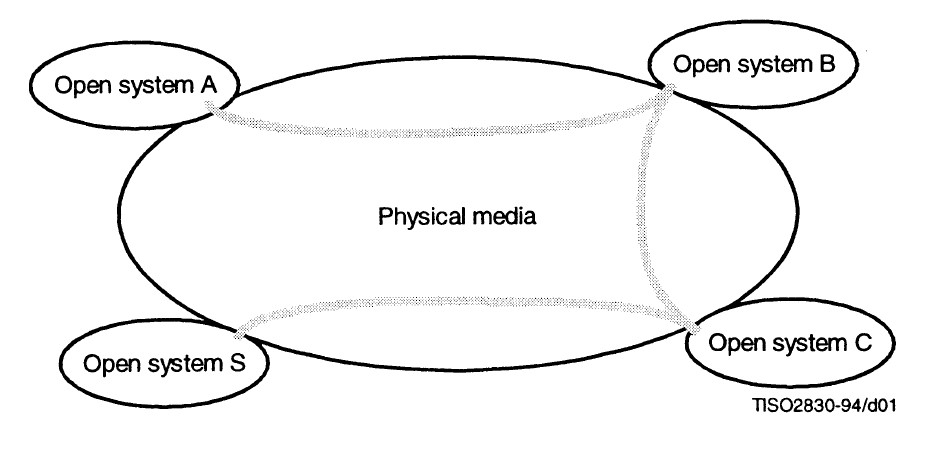
\includegraphics[width=\linewidth]{osianslutningar}
	\captionof{figure}{Förbindning av system i OSI-modellens\\ \\{\footnotesize Källa: \cite[s. 3]{iso74981}}}
\end{Figure}

OSI-modellen specificerar sju lager i arkitekturen för kommunikation:

\begin{enumerate}[label={\bfseries(\arabic*)}]
	\item Fysiska lagret: ansvarar för att sända och motta rå data mellan enheten och det fysiska mediumet
	\item Datalänk-lagret: ansvarar för kommunikation mellan noder och korrigering av fel som kan uppstå i fysiska lagret
	\item Nätverkslagret: ansvarar för överföring av datasekvenser --- paket --- mellan noder i nätverk
	\item Transportlagret: ansvarar för transport av datasekvenser från källa till destination utan kvalitetsförlust
	\item Sessionslagret: ansvarar för att hålla reda på dialoger mellan värder
	\item Presentationslagret: ansvarar för att hålla reda på kontext mellan applikationlager-entiteter 
	\item Applikationslagret: ansvarar för kommunikation med programvaran, lagret närmast användaren
\end{enumerate}

\subsection{Fältbussar och OSI-modellen}

PROFIBUS --- en vanlig standard för fältbussar --- följer standarden IEC 61158 (specifikt del två, IEC 61158-2) som beskriver den fysiska lagerspecifikationen för fältbussar. (\cite{profibuspowerplants}, \cite[s. 1083, \textit{IEC 61 158 Standard}]{fieldbustechindustrialautomation})

\begin{Figure}
	\centering
	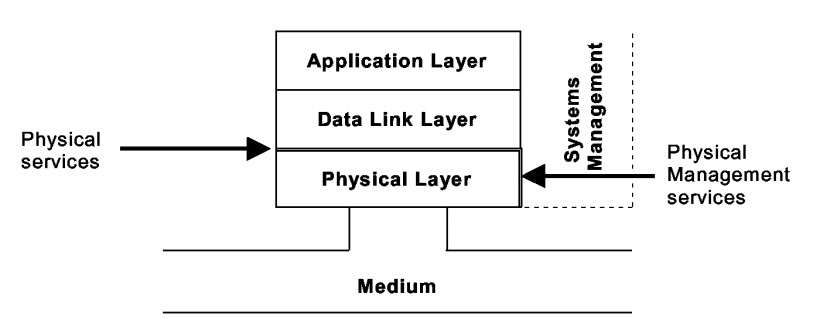
\includegraphics[width=\linewidth]{faltbusfysisktlager}
	\captionof{figure}{Relation till fysiska lagret av fältbussens nätverksarkitektur\\ \\{\footnotesize Källa: \cite[s. 884]{mapepa}}}
\end{Figure}

\end{multicols}

\clearpage\printbibliography

\end{document}
